\documentclass[titlepage]{article}

% For expanding the margins to be smaller than the default
\addtolength{\oddsidemargin}{-.875in}
\addtolength{\evensidemargin}{-.875in}
\addtolength{\textwidth}{1.75in}
\addtolength{\topmargin}{-.875in}
\addtolength{\textheight}{1.75in}

\pagestyle{plain}
\usepackage{color}
\usepackage{graphicx}

\begin{document}


\title{AZ-SMART Architecture Draft}
\author{Center for Urban Simulation and Policy Analysis\\University of Washington}
%\author{Jesse Ayers\\
%Paul Waddell\\
%David Socha}
\date{\today}
\maketitle

%\begin{abstract}
%Abstract
%\end{abstract}

\section{Proposed Architecture for AZ-SMART}
This document develops an architecture plan for the AZ-SMART project.  It is intended to provide an overview of the architecture from multiple perspectives: system, software, user interface, data and models.  Design choices are generally provided as recommendations, but in some cases two or more alternatives are presented for further discussion.  The intent is to update this document as design choices are finalized so that it can serve as an ongoing documentation effort.

\subsection{Functional Architecture Perspective}
The functional overview of the AZ-SMART system is depicted in Figure \ref{figWorkflow}, showing multiple activities connected in a sequential but also bi-directional workflow.  One can begin with the top-right of the diagram and work counter-clockwise to understand the intended workflow pattern.  An AZ-SMART user will begin with the GIS tasks of compiling a database in the Geodatabase that will contain all the needed information for the AZ-SMART system, with the exception of the travel model and a mid-level model that will be interfaced to AZ-SMART (in a later phase, the mid-level model is likely to become a component of AZ-SMART rather than an external process). 

As the database is assembled in the gepdatabase, including all land use layers, environmental, planning and political boundaries, development projects, and other related inputs, the AZ-SMART user will employ a suite of diagnostic tests to examine the database for missing, erroneous, and inconsistent data, and will use editing and validation tools to repair problems, and impute values for missing and erroneous data.  During this process, there would be considerable iteration between the data assembly step and the data diagnostic step, as some input data might be replaced or updated.  This step would also involve the assembly of metadata concerning the data sources, vintage, and any information developed on data quality.

The next step in the workflow is the development of models that are consistent with the database and can be used to allocate land uses to small areas (we discuss the form of the data in detail in the data subsection).  The models used by AZ-SMART will be configured to undertake land use allocation as described in the model subsection, and will be flexible with respect to the variables and weights (parameters) used.  The models themselves will be modular and flexible to allow ongoing refinement over time by AZ-SMART users as they gain insights into alternative means of doing the allocations.  This step also involves selecting the variables to use in each model component, and estimating model parameters statistically, or if desired, inputting parameters manually for some model components.  The tools for model estimation will be internal to the system, allowing ease of re-estimation if the user wishes to experiment with alternative specifications.  Diagnostics from model estimation, such as sensitivity to variables and correlation among variables, will be available to assess the robustness and sensitivity of each model component.  The user will also be able to compare observed to predicted data over an observed period if such data is available.  This model specification and calibration process may identify problems in the data, which will require moving back upstream in the workflow process to refine input data.

Once the models are estimated and the system calibrated to the users' satisfaction, the model system may be put into use. Putting the model into use requires the specification of one or more 'scenarios' that contain the input data that define the input conditions and assumptions for a run of the model system, including control totals, land development constraints, development projects, and transportation system.  These scenarios may involve graphical editing in the GIS environment, to edit boundaries of designated areas or to generate buffers or distances from specified features such as access points on the transportation system.  The scenario specification will also include controls for the interfacing of the travel model system (which years to run, what variables to pass, for example), and the mid-level land use model system or the control totals that have been generated by them.

The next step in the workflow is to run one or more scenarios over a forecast period defined by the scenarios.  This may be done in a batch mode that automates the entire modeling process from the loading of initial data for the base year, through multiple time steps and exchanges with the travel model, and possibly the mid-level model, until completion of the entire modeling period of 30 or more years (for example).  In other cases, the user may wish to run a scenario only for a portion of the intended forecast period, then stop the simulation to examine results, and possibly to make changes in the scenario assumptions that will shape the simulation in the next section of the forecast period.  Yet another possibility is that the user will see patterns in the results that are not desired, and decide to back up to the scenario specification stage, or even to the model specification stage, to make refinements and resume the process.

Typically the process of examining simulation results will involve creating indicators and extracts (or summaries) of the detailed simulation results.  We shall refer broadly to these as indicators.  The indicators may be simple aggregation of results, such as housing units or acres of each land use sector by zone, or RAZ.  Or they may involve computations that are more complex, such as estimating the remaining development capacity within each city.  The indicators may be produced as maps, or charts, or tables.  They may be of three types: snapshots (looking at an indicator for a single scenario and year), changes (usually from the base year to some forecast year), and differences (usually between a specific scenario and a baseline scenario for a selected year).  it is likely that many of these would be map indicators and be viewed in the GIS environment.

Simulation results may also be stored to the Geodatabase.  A user may wish to store either the full set of simulation results with all of the intermediate calculations needed to understand or even re-start a simulation from an intermediate year, or alternatively only a subset of specified results can be written to the Geodatabase for archiving and further visual examination.  The system will provide tools for both use cases.

This brings the workflow full circle to the top-right, where the data used as inputs and the data produced by the simulation may all be visually examined and edited.  Refinement of forecast results would be done at this stage also.  There are of course many possible variants on this workflow description, and theoretically one could draw connections among almost any pair of these task components, and the AZ-SMART system will support this kind of flexibility (but the diagram would be quite hard to interpret at that point).  The next section moves to the system architecture perspective.

\begin{figure}[h]
\begin{center}
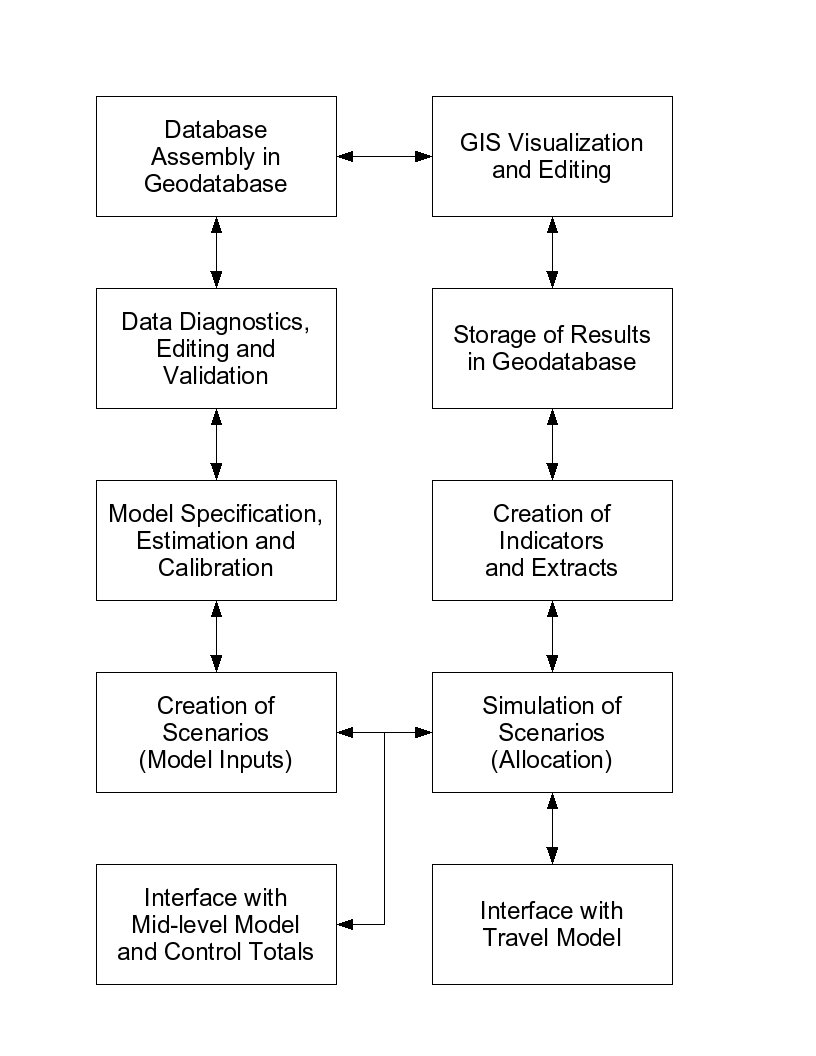
\includegraphics[scale=0.5]{figures/functional_diagram.png}
\caption{AZ-SMART Workflow Diagram}
\label{figWorkflow}
\end{center}
\end{figure}

\subsection{System Architecture Perspective}
This section provides a system perspective on AZ-SMART.  We describe a long-term perspective for the system, and suggest a first phase implementation.  The system is anticipated to evolve into a distributed configuration as depicted in Figure \ref{figSystem}, in which there are possibly different servers for the Geodatabase, running the land use model, running the travel model, and potentially a web server using ArcIMS or its successor.

Clients would be of the form of ArcGIS workstations, and OPUS Clients that would generally be on the same machine, integrated tightly with the ArcGIS user interface.  There may be situations in which a user wishes to run the OPUS GUI interface independently of ArcGIS, for example when focusing on model estimation, or at times when controlling simulation runs.  The interface between OPUS clients and servers would use networking infrastructure such as the Twisted Python framework.  

In the first phase, we expect that the OPUS client and server would be on the same machine as a an ArcGIS workstation, with multiple installations, one per user.  Data would be shared via the Geodatabase, and if desired also through a drive that is mapped from each of the clients to share the cache directory containing simulation results.

%\begin{center}
%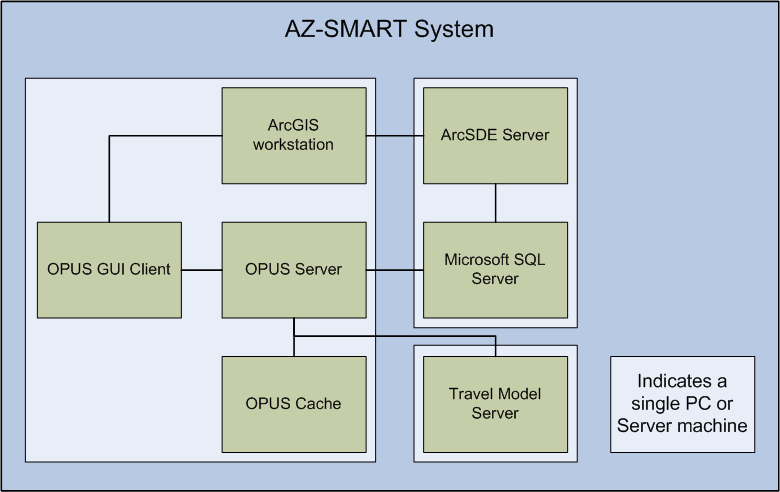
\includegraphics[scale=0.5]{'./figures/AZ-SMART_system_diagram.jpg'}
%\end{center}

\begin{figure}[h]
\begin{center}
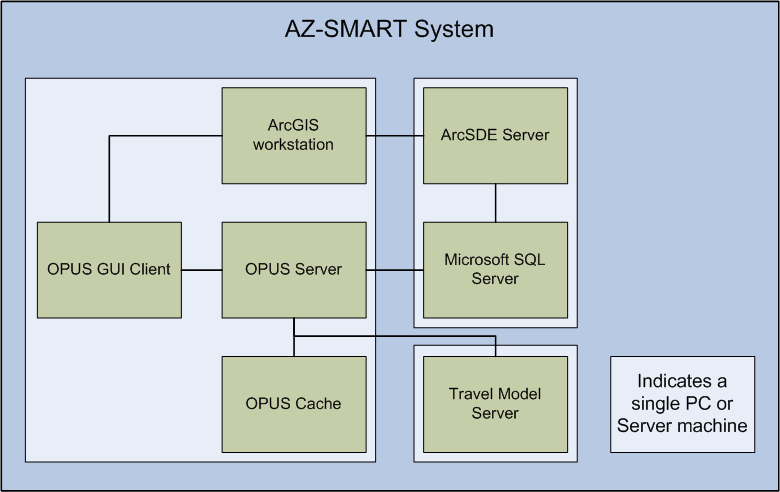
\includegraphics[scale=0.5]{figures/AZ-SMART_system_diagram.png}
\caption{AZ-SMART System Architecture}
\label{figSystem}
\end{center}
\end{figure}



\subsection{Data}

\subsubsection{Implementation}
Insert stuff about Geodatabase and OPUS Cache.
\subsubsection{Data Models}
Insert narrative and E-R diagrams.
\subsubsection{Data Diagnostics, Validation, and Imputation}
Insert stuff about data quality.

\subsection{Software}
Insert stuff about ArcGIS (ArcCatalog, ArcMap, ArcToolbox/ModelBuilder, dockable windows and toolbars), OPUS classes and methods, and how the two interact.

\subsection{Models}
Insert stuff about the model system.


\section{AZ-SMART Architecture Functional Requirements: Core Modules}
\emph{This section includes content from Appendix G of the AZ-SMART RFQ, along with with CUSPA's design recommendations for AZ-SMART core modules and including some questions that remain.  The purpose of this section is to begin to reconcile the design, implementation, and feature ideas presented in Appendix G with functionality within ArcGIS and Opus, and to identify the nature of new development needed.}

\subsection{Data Manager}
Overview
\begin{itemize}
\item Enhancements to ESRI ArcCatalog
\item At minimum, maintain current functionality

\emph{ArcCatalog will be used as the basis for the AZ-SMART Data Manager.  An AZ-SMART directory structure would organize these data, scripts, configurations and other components.}

\item Access to, development, and maintenance of all data
\item Create and track relationships (spatial and rule based) between datasets
\item Uses tools from Tool Manager
\item All data potentially used by more than one project. Examples include:
\begin{itemize}
\item Land Use Codes
\item Base Year
\item Allocation Sector Names
\item Legends
\item Symbol table associated with global variables
\end{itemize}

\emph{CUSPA proposes to create a custom AZ-SMART ArcCatalog Tree structure, that would be a dockable window containing and organizing the data and tools used in AZ-SMART.}


\item Metadata must be maintained for all datasets

\emph{Question for MAG: Need to jointly define the Metadata requirements and then devise a suitable design to address this need.}

\item Security

\emph{Question for MAG: Please identify user groups and security levels that are desired throughout the system and the scope of permissions for each user group.}

\item Consultant to recommend directory structure

\emph{A directory structure will be recommended and implemented in the AZ-SMART ArcCatalog Tree.}

\item Consultant to recommend and ultimately create data archiving procedures

\emph{Archiving procedures will be recommended once the database and all items needing to be archived are identified.}

\end{itemize}

%\begin{center}
%\includegraphics[scale=0.4]{AZ-SMART_DataManager_in_ArcCatalog.jpg}
%\includegraphics[scale=0.4]{AZ-SMART_DataManager_in_ArcMap.jpg}
%\end{center}

\begin{figure}
\begin{center}
\includegraphics[scale=0.3]{figures/AZ-SMART_DataManager_in_ArcCatalog.jpg}
\caption{AZ-SMART Data Manager in ArcCatalog}
\label{figDataManagerArcCatlog}
\end{center}
\end{figure}

\begin{figure}
\begin{center}
\includegraphics[scale=0.3]{figures/AZ-SMART_DataManager_in_ArcMap.jpg}
\caption{AZ-SMART Data Manager in ArcMap}
\label{figDataManagerArcMap}
\end{center}
\end{figure}


\subsection{Project Manager}

Overview

\emph{Projects are defined as the database and model configuration used to support running a variety of scenarios that would share data and model specifications and parameters.  Scenarios are defined as a set of input data, assumptions, and run configuration parameters used for a specific run of the model system.}  

\emph{CUSPA proposes to implement the Project Manager user interface as an OPUS GUI (developed using Envisage) that could be launched from an AZ-SMART Tool within ArcGIS.  Compared to an approach of using only native ArcGIS GUI tools, this approach will make it more feasible to implement several of the requirements listed below, particularly the last three items, which are very focused on control of model operations -- including during a simulation.  It would need to be implemented in a way that could inter-operate transparently with other tools in the Tool Manager and Data Manager components, as noted in the first requirement below. Some initial tests of this approach should be developed early in the project to flesh out this aspect of the user interface.}


\begin{itemize}
\item Create new projects and scenarios, or open projects and scenarios that have been created previously for further analysis
\item Links tools from Tool Manager with data from Data Manager using ESRI ModelBuilder concepts
\item Selects required components and limits execution of model to tools necessary for the scenario subset.
\item Accesses all data relevant to potentially more than one project via the Data Manager
\item Stores all data relevant to only that one project within a project. Examples include:
\begin{itemize}
\item Projection Years
\item Switches utilized in the project
\item Status of the project
\item File and database names etc.
\end{itemize}
\item Controls model execution: start, stop, and restart model execution
\item Access the status of a model while executing
\item Access various execution logs and error logs associated with a model run
\end{itemize}


\subsection{Tool Manager}
Overview
\begin{itemize}

\item Enhancements to ESRI ToolBox and ESRI ModelBuilder

\emph{ESRI ArcToolbox and ModelBuilder will be used as the basis for the majority of the GUI for AZ-SMART.  It will be enhanced by adding tools that leverage OPUS and UrbanSim functionality, generally through the OPUS GUI).}

\item Will have an indexing system by which end-users can find appropriate tools relevant to their needs

\emph{The built-in ArcToolbox indexing system will be used for this purpose.}

\item Accesses Script Editor to code/implement tools

\emph{The built-in editing functionality for Python will be used for this purpose.}

\item Uses ModelBuilder for computer-aided programming (i.e., data flow chart graphical interface)

\emph{The built-in ModelBuilder functionality will be used for this purpose.}

\item Manage scripts: open, create, copy, delete, edit tools and their properties

\emph{The built-in ArcToolbox functionality for managing scripts will be utilized here.  This is accessible via context-menu selections at the toolset and tool level in ArcToolbox.}

\item Multiple security levels

\emph{Question for MAG: Please identify user groups and security levels that are desired throughout the system and the scope of permissions for each user group.}

\item Multi-user system

\emph{The system will be designed to use the ArcSDE multi-user environment with Microsoft SQL Server, which provides multi-user capabilities.}

\item Ability to share tool based on properties assigned

\emph{Question for MAG: This functionality needs further clarification about what is needed.  It may be possible to store tools in the Geodatabase, providing security and sharing capabilities within.}

\item Will perform conditionals and loops

\emph{The built-in ArcToolbox and ModelBuilder functionality will be used to perform conditionals and loops, augmented by Python and OPUS capabilities.}

\item Unless specified, all tools should be capable of accepting input from user, script, output from other tools, or a database

\emph{Tools will be constructed to meet this qualification.}

\item Consultant to recommend and ultimately create:
\begin{itemize}
\item Tool archiving procedures

\emph{This will require the use of a version control system such as Subversion. A Subversion repository has been set up for this project at CUSPA. An existing tool for accessing Subversion from Python could be linked from the user interface (www.pysvn.tigris.org). }

\item Definition and management of production and development versions

\emph{This could be accomplised by having two branches in the Subversion repostitory, one for production code, one for development code.}

\item Prevention of the inadvertent modification and/or deletion of tools referenced elsewhere in the system

\emph{This could be accomplished by placing relevant Toolboxes and Toolsets in a 'read-only' location.}

\end{itemize}
\end{itemize}

Example Tools from MAG

\subsubsection{Land Use Editor}

Overview

\begin{itemize}

\item An ArcGIS application toolbar that provides controls specifically suited for editing and managing land use databases

\emph{CUSPA proposes to use ArcGIS built-in editing functionality for editing of spatial features (e.g. existing land use, development projects), augmented by a toolset.  If there is remaining functionality in SAM-IM that is not already addressed by built-in ArcGIS editing, then an ArcMap toolbar would be created to meet these needs.}

\item Maintains planar polygon topology/grid; Data model aware; Performs validation and domain checking

\emph{CUSPA proposes to utilize built-in geodatabase functionality for maintaining topology, domain checking, etc.  There are existing tools (e.g. Geodatabase designer 2) that can address these requirements.}

\item Advanced wizards for manipulating, validating, and assembling land use themes using interactive input and configurable rules

\emph{CUSPA proposes to focus on developing tools and ModelBuilder models to meet these needs.}

\item Aggregation of parcels based on predefined rules (e.g. eliminate minor roads)

\item Subdivision of parcels or polygons based on predefined rules

\emph{The aggregation and subdivision of parcels or polygons are two complex tasks that need further design work and an assessment of alternative approaches.}

\item Variable sized grids with associated attribute data (e.g. areas with high vs. low resolution for modeling and analysis)

\emph{CUSPA understands the potential benefits of variable sized grids for preserving small polygons in dense core of the urban area and avoiding wasted storage using small gridcells to represent large polygons in the urban periphery.  However, implementing variable resolution grids is potentially a research project with considerable risk.  Further discussion of the objectives, alternative strategies, and risks associated with these is needed.}

\item Can access data in Data Manager or Project Manager

\emph{CUSPA proposes that all data in the geodatabase will be directly accessible in Data Manager and/or Project Manager as appropriate.  Data generated during a simulation would be accessible in Data Manager and/or Project Manager through the use of tools to copy the data into the geodatabase or other tabular formats.}

\item Consistency checking across multiple themes

\emph{Tools would be developed to check for consistency within and across themes as needed.}

\item Summary and indicator statistics

\emph{This would be built using the Opus indicator framework.}

\item Completely configurable to suit any land use data model, coding scheme, and installation

\emph{AZ-SMART will be designed to be highly modular and configurable and will use the flexibility inherent in the Opus sytesm.}

\item Similar to current editing capabilities in SAM-IM

\emph{Existing ArcMap functionality will be utilized to provide this functionality.}

\end{itemize}

\subsubsection{Land Use and Socioeconomic Synthesizer}

CUSPA proposes to develop tools for creating, manipulating, and synthesizing a base year database in the ArcToolbox/ModelBuilder environment.

\begin{itemize}

\item For creating and populating the base year (e.g., 2000) land use database by assembling multiple sources.

\item For creating projected land use and socioeconomic datasets based on configurable rules.

\emph{This would be done by implementing models in Opus and allowing them to be configured and run within ArcGIS. }

\end{itemize}

\subsubsection{Calibration and Validation}

\begin{itemize}

\item Utilities for creating calibration data sets based on user supplied specifications
\item Use 3rd party programs to perform regression analysis (e.g., ALOGIT, SPSS)
\item Utilities for validating calibrated model data against observed data

\emph{Opus includes tools for creating estimation datasets, estimating parameters of multiple regression and discrete choice models.  These tools would be used for specifying and estimating models in AZ-SMART.  Model validation will be supported by tools to compare predicted and observed data and visualize patterns of error in the results.}

\end{itemize}

\subsubsection{Analysis, Visualization, and Reporting}

\begin{itemize}
\item A spatial calculator to perform computations on socioeconomic databases, examples:
\begin{itemize}
\item Incorporate data from external sources;
\item Prorate projections to polygons based on a demographic property;
\item Drop point data into polygons (TAZ or land use polygons);
\item Perform row and column normalization and matrix balancing
\item Automatically summarize land use themes according to other polygon geographies (e.g., TAZs)
\item Calculate socioeconomic and land use statistics (population, employment, acres by type) for user defined areas based on geospatial rules.
\item Compute indicators and measures on land use or other polygon geographies (e.g., job-housing balance).

\emph{Question to MAG: The needs detailed in this section warrant further discussion.  CUSPA anticipates that some of this functionality will be handled by ArcGIS and Opus functionality.}

\end{itemize}

\item Capability to export tables to any file format, including custom format text files needed by travel models as well as ArcIMS; Users can define and save various file formats into a library of templates, and recall them for later exports.

\emph{The system will provide a capacity for the user to define the particular data to be exported, variables, their sequence, the file format, and location.  Export formats would include dbase, SQL server, ASCII (tab delimited, comma delimited, and fixed format). Question for MAG: Does this address the needs for ArcIMS?}

\item Provides methods by which end-users can define series of thematic maps to be generated automatically
\item Provides methods by which end-users can define statistical tables and reports to be generated automatically

\emph{The process of generating indicators and displaying them on a user configured base map will be automated.}

\end{itemize}

\subsubsection{Data Manipulation and Conversion Utilities}

\begin{itemize}

\item Data available in a number of different file/DBMS formats: MS Excel spreadsheets, MS Access, Formatted ASCII files, Geodatabases, MySQL, etc.
\item A library of utilities for accessing/converting data from one form to another so that it can be accessed directly by tools implementing models

\emph{The system will support accessing and converting data among various data formats including but not limited to those formats listed above.}

\end{itemize}

\subsubsection{Accessibility}

\begin{itemize}

\item Consultant to recommend and implement methodology or methodologies for travel times from geography to geography. Examples include:
\begin{itemize}
\item Accesses travel times directly from third party systems used by MPOs (e.g., EMME/2, Cube)
\item Accesses travel times directly from modified third party systems using larger levels of geography
\item Creates travel times within AZ-SMART without using 3rd party systems
\end{itemize}

\emph{CUSPA proposes to develop an interface to the forthcoming MAG TransCAD travel model if it is availabe within the timeframe of the AZ-SMART phase 1 project.  It may be desirable to develop a sketch-level (fast running) travel model in later phases.}

\end{itemize}

\subsubsection{Submodels}

\emph{CUSPA will need to work with MAG staff to develop clear specifications for sub models to be developed.}


\subsubsection{Site Suitability Tools}
\begin{itemize}
\item Characterizes potential development sites throughout a region with respect to its suitability for development;
\item A toolbox for portraying site characteristics from other GIS users (e.g., age and condition of structure, land value, proximity to highways, distance to developed land, residential market within 3 miles, etc.)
\item Creates input datasets used in calibration
\item An important component of allocation of lands during a projection, using calibrated factors

\emph{CUSPA proposes to develop a set of tools organized within a Site Suitability Toolset to use themes for planned land use and various environmental or other features that would be used in determining suitability for each land use sector.  These would be used to determine the capacity for development of each corresponding building type, such as Single Family units, Multi-family units, Office Sqft, etc, and could account for planning constraints such as minimum or maximum floor-area ratio (FAR) regulations.}

\end{itemize}

\subsubsection{Allocation Tool}

\emph{This section describes functional requirements for a model system used to allocate land uses.  CUSPA proposes to use existing functionality in OPUS to implement these models.  The models and their specification would be configurable using dialog boxes or forms, and connected using a Model Builder style interface within the proposed OPUS GUI.  Features described below will be incorporated into these tools.  Comments inserted below are for clarification of the functional requirements.  A more complete description of the design of the Allocation Models is provided in a subsequent section.}

\begin{itemize}
\item A key tool for projecting growth in a region
\item At minimum, maintain current functionality of SAM-IM

\emph{The intent is to provide at least comparable functionality, though not using exactly the same approach.}

\item Process works by selecting lands, among candidates, to be built in order to absorb growth based on an evaluation of their inherent site suitability characteristics
\item Features include but are not limited to:
\begin{itemize}
\item Observes constraint layers that prohibit development due to environmental or policy factors
\item Observes general plan layers that designate acceptable conforming land uses and densities
\item Accepts any land use coding scheme that the user defines
\item Allocation sectors (variables of interest for projections) are user-defined
\item Sectors are allocated in a user-defined sequence.
\item Mechanism by which large development tracts are subdivided into parcels appropriate in size for the development considered

\emph{Note earlier comments that aggregation and subdivision will require substantial design work and further discussion.}

\item Ability to observe adopted land use plans and densities on a polygon/grid basis
\item Development Velocity Curve dictates the pace at which developments are built
\item Observes regional control totals of growth, or growth forecasts for subareas, as defined
\item Address "mixed use" polygons
\item Address redevelopment and demolition
\end{itemize}
\item Same process can be used, with different inputs, for vacating lands due to demolition and redevelopment
\item Controlled by a number of different switches and rules supplied by the user that control how the allocation process specifically works
\item Driven by a set of projected control totals of population and employment change that apply to the entire region or subareas of it
\item Can control subarea growth at different geographic levels
\item Capability for  "gravity effects" model projection mechanisms reacting to measures of accessibility, land use constraints and opportunities, growth trends, and other socioeconomic attributes
\item Provides specific treatment of known developments scheduled to be underway
\item Provides support for analysis of scenarios:
\begin{itemize}
\item Generates alternative scenarios of land use and socioeconomic projections
\item Ability to work on complete area or revision-areas (sub-parts of complete modeling area)
\item Interactive designation of  "revision areas"; Capability to manipulate both polygon and grid
\item Migrates changes in downstream years; that is, changes made to a 2010 forecast migrated automatically to subsequent years;
\end{itemize}
\item Provides different ways to react:
\begin{itemize}
\item When build-out conditions are reached in individual subareas
\item How active developments are treated
\item With respect to policy initiatives
\item To demolition and redevelopment 
\end{itemize}
\item Different applications of the Allocation procedure in the projection model stream:
\begin{itemize}
\item Regular production projections
\item "Min-Max" procedure to create set of floors and ceilings to estimate reasonable growth potential
\item "Scenario Builder" enabling analysis of changes to land use and other policy variables. 
\end{itemize}
\end{itemize}



\section{Nouns and Verbs}

Following are lists of the nouns and verbs identified by reading Appendix G.  (We are still assembling this.)  We expect that each of these nouns will correspond to a class in our object-oriented system, so understanding the nouns and verbs is important for understanding what we are building.  In general, a noun corresponds to a class, and a verb corresponds to a method of that class.  Classes generally have additional methods and properties for internal use in the system.

\subsection{Nouns from Appendix G}

\begin{itemize}
  \item Meta-data.  Every noun has meta-data that covers its who, what, when, where, and why.  In addition, a user may enter arbitrary key, value pairs?
  \item Project.  A project defines the geographical scope, set of issues of concern, time-frame desired, etc. for a specific investigation into some set of issues.
  \item Scenario.  A scenario is a particular configuration of input data, assumptions, and models to run to test a particular alternative future.  Every project will eventually have at least one scenario.  You can only 'run' scenarios.
  \item Scenario run.  Information about the running of a scenario.  This includes meta-data and simulation results.  Simulation results may be viewed by indicators.
  \item Indicator definition.  Specification of how to compute a particular indicator.  
  \begin{itemize}
	  \item Map indicator definition.
	  \item Table indicator definition.
	  \item Chart indicator definition.
	  \item Report indicator definition.  This may consist of meta-data as well as a collection of other indicators (maps, tables, charts, etc.).
  \end{itemize}
  \item Indicator result.  Result of running an indicator or a scenario run.  Synonym: prediction?
  \begin{itemize}
	  \item Map indicator results.
	  \item Table indicator results.
	  \item Chart indicator results.
	  \item Report indicator results.  
  \end{itemize}
  \item Indicator set.  Multiple indicators.  Allows multiple indicators to be operated on as a unit (e.g. create all of these).
  \item Data-flow diagram.  This is a ``model'' in ModelBuilder.  It is a visual representation of a data flow from a set of data sources, through a set of actions, to a set of data outputs.  Includes conditionals and loops.
  \item Scenario subset.  What is this?
  \item Model. 
  \item Development.
  \item Custom procedure.  For instance, a script, or a data-flow diagram.
  \item Tool.  A software component that has a user interface.
  \item Software component.
  \item Data input.
  \item Data output.
  \item \ldots
\end{itemize}

\subsection{Verbs from Appendix G}

\begin{itemize}
  \item New.  Synonym: create.
  \item Save.
  \item Edit.
  \item Open/View.
  \item Delete.
  \item Copy.
  \item Run.  Synonym: project.
  \item Manage.  What does this mean?
  \item Analyze.
  \item \ldots
\end{itemize}

\subsection{Combining Nouns and Verbs}

These nouns and verbs could suggest the following menu items or tools that correspond to features or feature categories:

\begin{itemize}
  \item Project
  \begin{itemize}
	  \item New project.
	  \item Open project.
	  \item Save project.
	  \item Modify project.
	  \item Copy project.
	  \item Delete project.
	\end{itemize}
	
  \item Scenario 
  \begin{itemize}
	  \item New scenario.  Linked to a particular project.
	  \item Open scenario.
	  \item Save scenario.
	  \item Modify scenario.
	  \item Copy scenario.
	  \item Run scenario.  Produces a scenario run.
	  \item Delete scenario.
	\end{itemize}
	
  \item Scenario Run 
  \begin{itemize}
	  \item Open scenario run (read only?).
	  \item Delete all or part of a scenario run.  For instance, to prepare to re-run starting in 2020.
	  \item Copy all or part of a scenario run.  For instance, to send to a colleague.
	\end{itemize}
	
  \item Indicator Definition 
  \begin{itemize}
	  \item New indicator definition.  Defines how to compute an indicator results.
	  \item Open indicator definition.
	  \item Save indicator definition.
	  \item Delete indicator definition.
	\end{itemize}
	
  \item Indicator Results 
  \begin{itemize}
	  \item New indicator results.  Compute an indicator results from an indicator definition.
	  \item Open/View indicator results.
	  \item \ldots
	\end{itemize}
	
  \item Indicator Set 
  \begin{itemize}
	  \item Create an indicator set.
	  \item View/edit/save an indicator set.
  \end{itemize}
  
  \item Data-flow Diagram.  
  \begin{itemize}
    \item New data-flow diagram.
    \item \ldots
    \item Edit component from diagram.  A componet may be a node or an edge.  For instance, right-click on a data-source to set its properties.
    \item Run data-flow diagram.  
    \item Validate data-flow diagram.
    \item Step-over data-flow diagram.  Runs next step in diagram.
    \item Step-into current node.  During simulation.
    \item Set breakpoint.  Execution will stop just before executing the component that has the breakpoint.
    \item Open selected node.  Opens editor for the node, which may be a data-flow diagram itself.
    \item Open selected edge.  Opens property editor for the edge.
    \item Select node.  To edit, open, move, delete, etc.
  \end{itemize}
\end{itemize}

\end{document}